%%%%%%%%%%%%%%%%%%%%%%%%%%%%%%%%%%%%%%%%%%%%%%%%%%%%%%%%%%%%%%%%%%%%%%%%%%%%
%    This LaTeX source was automatically generated by outlinebeamer.pl     %
%                                                                          %
%   Remember that most changes should be made to the outline source file   %
% changes to this file will be overwritten when the file gets regenerated  %
%                                                                          %
%                  outlinebeamer - Outline Beamer Class Presentation Maker %
%                                    http://outlinebeamer.sourceforge.net/ %
%%%%%%%%%%%%%%%%%%%%%%%%%%%%%%%%%%%%%%%%%%%%%%%%%%%%%%%%%%%%%%%%%%%%%%%%%%%%
\documentclass{beamer}
\newcommand{\Code}[1]{\textsf{#1}}
\newcommand{\cello}{\textsf{Cello}}
\newcommand{\enzo}{\textsf{Enzo}}
\usetheme{Copenhagen}
\usecolortheme{default}
\newcommand{\code}[1]{\texttt{#1}}
\newcommand{\us}[1]{\color{blue}{#1}}
\newcommand{\them}[1]{\color{red}{#1}}
\newcommand{\newus}[1]{\color{magenta}{#1}}
\newcommand{\good}{\textcolor{green}{\smiley}}
\newcommand{\bad}{\textcolor{red}{\frownie}}
\newcommand{\colorcode}[1]{\textcolor{blue}{\code{#1}}}
\def\enhance<#1>{%
 \temporal<#1>{\color{lightgray}}{\color{black}}{\color{gray}}}
\def\enhanceus<#1>{%
 \temporal<#1>{\color{lightgray}}{\color{blue}}{\color{blue}}}
\def\enhancenewus<#1>{%
 \temporal<#1>{\color{lightgray}}{\color{magenta}}{\color{magenta}}}
\def\enhancethem<#1>{%
 \temporal<#1>{\color{lightgray}}{\color{red}}{\color{red}}}
%======================================================================
\title[The \cello\ Project]
      {The \cello\ Project \\ \small{\enzo: The Next Generation}}
\author[James Bordner]{\small Laboratory for Computational Astrophysics \\ San Diego Supercomputer Center \\ University of California, San Diego \\ \ \\ James Bordner}
\date{\today}
\begin{document}
\frame{\titlepage}
\frame{\tableofcontents}
\AtBeginSubsection[]
{
%------------------------------------------------------------------------
  \begin{frame}<beamer>
    \tableofcontents[currentsection,currentsubsection]
  \end{frame}
}



\section{Overview}
%------------------------------------------------------------------------
    \begin{frame}[fragile] \frametitle{Outline}
      \begin{itemize}
        \item Overview
        \item User Perspective
        \begin{itemize}
          \item Parameter files
          \item Examples
        \end{itemize}
        \item AMR Data Structures
        \begin{itemize}
          \item Other AMR codes
          \item Cello Patch AMR
          \item Cello Tree AMR
        \end{itemize}
        \item Code Architecture
        \begin{itemize}
          \item Components
          \item Hardware interface components
          \item Method component
          \item Data structures
          \item Control
        \end{itemize}
      \end{itemize}
\end{frame}

%------------------------------------------------------------------------
    \begin{frame}[fragile] \frametitle{Goals}
      \begin{itemize}
        \item \enzo: The Next Generation
        \item Computational science tool for next 10+ years
        \item Many competing design goals:
        \begin{itemize}
          \item Scalable to O($10^{5+}$)  cores
          \item Easy to use, modify, adapt, maintain
          \item Quality control
          \item \textit{Science capabilities}
        \end{itemize}
      \end{itemize}
\end{frame}

%------------------------------------------------------------------------
    \begin{frame}[fragile] \frametitle{Target Classes of Users}
      \begin{itemize}
        \item \enhance<1>\textbf<1>{Students}
        \begin{itemize}
          \item \enhance<1>easy to define problem, run, and analyze
          \item \enhance<1>minimal software-related ``gotcha's''
        \end{itemize}
        \item \enhance<2>\textbf<2>{Physics experts}
        \begin{itemize}
          \item \enhance<2>deep control of physics parameters
          \item \enhance<2>flexible problem set up for wide range of problems
        \end{itemize}
        \item \enhance<3>\textbf<3>{Numerical experts}
        \begin{itemize}
          \item \enhance<3>deep control of method parameters
          \item \enhance<3>easy to incorporate new methods
        \end{itemize}
        \item \enhance<4>\textbf<4>{Computing experts}
        \begin{itemize}
          \item \enhance<4>deep control of data structures
          \item \enhance<4>AMR, parallelization, data distribution, blocking/padding
        \end{itemize}
      \end{itemize}
\end{frame}

%------------------------------------------------------------------------
    \begin{frame}[fragile] \frametitle{Target Classes of Problems}
More AMR $\rightarrow$ more data dependencies $\rightarrow$ less parallelism
      \begin{itemize}
        \item \enhance<1>\textbf{Single-resolution (``unigrid'')}
        \begin{itemize}
          \item  \enhance<1>Parallelizes fully
          \item  \enhance<1>\enzo\ does well, but still room for improvement
        \end{itemize}
        \item \enhance<2>\textbf{Shallow multi-resolution}
        \item \enhance<3>\textbf{Deep multi-resolution}
        \item \enhance<4>\textbf{\textit{Extreme} multi-resolution}
        \begin{itemize}
          \item \enhance<4>Most difficult to parallelize effectively
          \item \enhance<4>\enzo\ does not scale well with hierarchy depth
        \end{itemize}
      \end{itemize}
\end{frame}

%------------------------------------------------------------------------
    \begin{frame}[fragile] \frametitle{Petascale Performance Issues}
      \begin{itemize}
        \item Synchronization
        \item Parallel task control
        \begin{itemize}
          \item Large enough to be efficient
          \item Small enough for sufficient parallelism
        \end{itemize}
        \item Task scheduling
        \begin{itemize}
          \item Static scheduling with dynamic load balancing
          \item Dynamic scheduling with job migration
          \item Controlable via, e.g., CHARM++
        \end{itemize}
        \item Load balancing
        \item Software resiliency
        \item Restarts
        \item AMR performance issues
        \begin{itemize}
          \item Finding patch neighbors
          \item Parallel gridding algorithms
          \item Memory usage
          \item Elliptic solves: gravity / radiation
        \end{itemize}
      \end{itemize}
\end{frame}

%----------------------------------------------------------------------
\begin{frame}
\frametitle{Summary of changes compared to \enzo}
\begin{itemize}
\item Overhauled parallel distributed data structures
\item Improved AMR approach(es)
\begin{itemize}
\item  Patch-based and tree-based AMR have advantages/disadvantages
\item  Implement both
\end{itemize}
\item Improved definition and control of parallel tasks
\begin{itemize}
\item Maintain pool of parallel tasks (CHARM++?)
\item Flexible data distribution
\item Smarter  data re-distribution
\item Multiple choices for parallelism (MPI-[12], OMP, UPC)
\end{itemize}
\item Improved problem specification scope and depth of control
\item More rigorous software development methodology
\end{itemize}
\end{frame}
%------------------------------------------------------------------------
    \begin{frame}[fragile] \frametitle{Parameter Files}
\end{frame}

%------------------------------------------------------------------------
    \begin{frame}[fragile] \frametitle{Parameter File: Shock Pool draft}
 \footnotesize
\begin{block}{Shock Pool: Domain, Grid, and Field parameters}
      \begin{verbatim}
  # Define the domain to be the 1D interval from 0 to 1

  Domain { range = [0.0, 1.0] }

  # The grid is a unigrid array of 100 cells 
  # parallelized using MPI+OpenMP (!)
 
  Grid { size = [100]; parallel = [mpi,omp] }

  # define field properties

  Field pressure { floor = 1.0e-6 }
  Field density  { floor = 1.0e-6 }
      \end{verbatim}
\end{block}
\end{frame}

%------------------------------------------------------------------------
    \begin{frame}[fragile] \frametitle{Parameter File: Shock Pool draft}
 \footnotesize
\begin{block}{Shock Pool: Method and Boundary}
      \begin{verbatim}
  # Physics method is ppm hydro
 
  Method ppm {
      gamma     = 1.4;
      courant   = 0.5;
      diffusion = false
  }
 
  # Define boundary conditions
 
  Boundary { type = reflecting }
      \end{verbatim}
\end{block}
\end{frame}

%------------------------------------------------------------------------
    \begin{frame}[fragile] \frametitle{Parameter File: Shock Pool draft}
 \footnotesize
\begin{block}{Shock Pool: Initial and Stopping}
      \begin{verbatim}
  # Define initial conditions
 
  Initial {
     pressure   = [1.0,   x <= 0.5,
                   0.125, x > 0.5];
     density    = [1.0, x <= 0.5,
                   0.1]; # (implicit else)
     velocity_x = 0
  }
 
  # Define stopping criteria
 
  Stopping {
     time  = 0.251;
     cycle = 10000
  }
      \end{verbatim}
\end{block}
\end{frame}

%------------------------------------------------------------------------
    \begin{frame}[fragile] \frametitle{Software Components}
\centerline{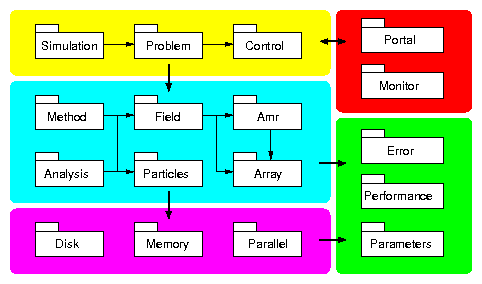
\includegraphics[width=4in]{components.png}}
\end{frame}

%------------------------------------------------------------------------
    \begin{frame}[fragile] \frametitle{Software Components: Hardware}
\end{frame}

%------------------------------------------------------------------------
    \begin{frame}[fragile] \frametitle{Software Components: AMR data structures}
\end{frame}

%------------------------------------------------------------------------
    \begin{frame}[fragile] \frametitle{Review of AMR Approaches}
    \footnotesize
      \begin{tabular}{|l|ccc|cc|}
\hline
    &  \textbf{Enzo} & \textbf{Chombo} & \textbf{Paramesh} & \textbf{Cello-patch} & \textbf{Cello-tree} \\  \hline
    \textbf{Refinement} &  \enhanceus<2>{patch} & \enhancethem<3>{patch} &  \enhancethem<4>{tree} & \enhancenewus<5>{patch} & \enhancenewus<6>{tree}  \\
    \textbf{Tree type} & \enhanceus<2>{none} & \enhancethem<3>{octree} & \enhancethem<4>{octree} & \enhancenewus<5>{octree} & \enhancenewus<6>{octree++} \\  \hline
    \textbf{Parents} & \enhanceus<2>{single} & \enhancethem<3>{multiple} & \enhancethem<4>{single} &   \enhancenewus<5>{multiple} & \enhancenewus<6>{single} \\
    \textbf{Children} & \enhanceus<2>{variable} & \enhancethem<3>{variable} & \enhancethem<4>{constant} & \enhancenewus<5>{variable} & \enhancenewus<6>{limited} \\
    \textbf{Neighbors} & \enhanceus<2>{variable} & \enhancethem<3>{variable} & \enhancethem<4>{limited} & \enhancenewus<5>{variable} & \enhancenewus<6>{limited} \\\hline
    \textbf{Level jumps} & \enhanceus<2>{ yes} &    \enhancethem<3>{no} &      \enhancethem<4>{no}    &   \enhancenewus<5>{no} & \enhancenewus<6>{no} \\
    \textbf{Symmetric} & \enhanceus<2>{no} &  \enhancethem<3>{yes} &  \enhancethem<4>{yes} &  \enhancenewus<5>{yes} & \enhancenewus<6>{yes} \\\hline
    \textbf{Patch shape} & \enhanceus<2>{  variable} & \enhancethem<3>{variable} &  \enhancethem<4>{constant} & \enhancenewus<5>{variable} & \enhancenewus<6>{constant} \\
    \textbf{Patch size} & \enhanceus<2>{  variable} & \enhancethem<3>{variable} &  \enhancethem<4>{constant} & \enhancenewus<5>{variable} &\enhancenewus<6>{limited}  \\ \hline
      \end{tabular}
\end{frame}

%------------------------------------------------------------------------
    \begin{frame}[fragile] \frametitle{Software Components: \code{Array} + \code{Amr}}
\end{frame}

%------------------------------------------------------------------------
    \begin{frame}[fragile] \frametitle{Software Components: \code{Array}}
\end{frame}

%----------------------------------------------------------------------
\begin{frame}
\frametitle{\code{Array} class}

\begin{itemize}
\item Conceptually a Fortran-like array
\item Data distributed via MPI-[12], OMP, [UPC]
\item Data layout may be blocked / padded for cache
\item Interface between high-level C++ and low-level Fortran/C
\end{itemize}
\end{frame}
%----------------------------------------------------------------------
\begin{frame}
\frametitle{\code{Array} class}

\begin{minipage}{1.8in}
\begin{itemize}
\item[]<1->
\includegraphics[width=0.4in]{array-serial.png} \ \ \code{ArraySerial}
\item[]<2->
\includegraphics[width=0.4in]{array-block.png} \ \ \code{ArrayBlock}
\item[]<3->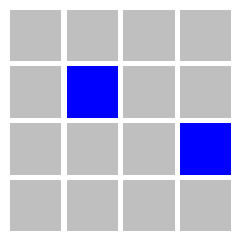
\includegraphics[width=0.4in]{array-mpi.png} \ \ \code{ArrayMpi}
\end{itemize}
\end{minipage} \ 
\begin{minipage}{2in}
\begin{itemize}
\item[]<4->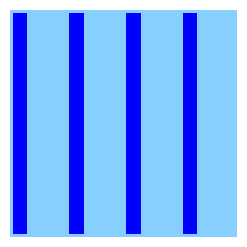
\includegraphics[width=0.4in]{array-omp.png} \ \ \code{ArrayOmp}
\item[]<5->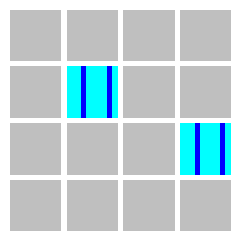
\includegraphics[width=0.4in]{array-mpi-omp.png} \ \ \code{ArrayMpiOmp}
\item[]<6->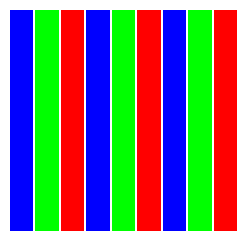
\includegraphics[width=0.4in]{array-interleave.png} \ \ \code{ArrayInterleave}
\end{itemize}
\end{minipage}

\end{frame}
%----------------------------------------------------------------------
%------------------------------------------------------------------------
    \begin{frame}[fragile] \frametitle{Software Components: \code{Amr}}
\end{frame}

%------------------------------------------------------------------------
    \begin{frame}[fragile] \frametitle{Control}
      \begin{itemize}
        \item Task: advance grid patch one timestep
        \item Dependencies: boundary values
        \item Dynamic task scheduling
        \begin{itemize}
          \item No artificial dependencies imposed
          \item Patches in different levels can advance concurrently
          \item CHARM++ would be helpful
        \end{itemize}
      \end{itemize}
\end{frame}

%------------------------------------------------------------------------
    \begin{frame}[fragile] \frametitle{Local adaptive time-stepping}
      \begin{itemize}
        \item \enzo\ supports adaptive time-stepping between levels
        \item Fully adaptive time-stepping option
        \begin{itemize}
          \item No global timestep restriction
          \item No global synchronization
        \end{itemize}
        \item Uniform time-stepping option
        \begin{itemize}
          \item High parallel efficiency
          \item Simplified code
          \item Happy
        \end{itemize}
      \end{itemize}
\end{frame}

%------------------------------------------------------------------------
    \begin{frame}[fragile] \frametitle{Particle positions}
      \begin{itemize}
        \item Particles are associated with a patch
        \item Represent particles in patch-local coordinates
        \item Simple coordinate transformation when particles migrate
        \item Single-precision sufficient
        \item Global coordinates
      \end{itemize}
\end{frame}

%------------------------------------------------------------------------
    \begin{frame}[fragile] \frametitle{Hierarchical Load balancing}
\end{frame}

%------------------------------------------------------------------------
    \begin{frame}[fragile] \frametitle{Precision issues: Particles}
      \begin{itemize}
        \item Use local coordinate system when possible
        \begin{itemize}
          \item Particles coordinates [0:1] in containing grid patch
          \item Simple coordinate transform when containing patch changes
          \item Single precision sufficient
          \begin{itemize}
            \item Save memory
            \item Save time
          \end{itemize}
        \end{itemize}
      \end{itemize}
\end{frame}

%------------------------------------------------------------------------
    \begin{frame}[fragile] \frametitle{Precision issues: Grids}
      \begin{itemize}
        \item Define grid location only relative to neighboring grid
        \item 32-bit integerss always sufficient
        \item No global tree structure
        \item Issues
        \begin{itemize}
          \item Load balancing
          \begin{itemize}
            \item CHARM++
          \end{itemize}
          \item Re-gridding
          \begin{itemize}
            \item local algorithm
          \end{itemize}
          \item Global time step
        \end{itemize}
        \item High scalability
      \end{itemize}
\end{frame}

%------------------------------------------------------------------------
    \begin{frame}[fragile] \frametitle{Gravity}
      \begin{itemize}
        \item Hypre insufficient
        \begin{itemize}
          \item Best method FAC is unusable
        \end{itemize}
        \item Write own FAC
        \item Chombo group is on top of this
      \end{itemize}
\end{frame}

%------------------------------------------------------------------------
    \begin{frame}[fragile] \frametitle{AMR: point-source test with full $2^d$-trees}
\begin{minipage}{2.5in}
\includegraphics<1>[width=2.5in]{dots.png}
\includegraphics<2>[width=2.5in]{dots-4-0.png}
\includegraphics<3>[width=2.5in]{dots-4-1.png}
\includegraphics<4>[width=2.5in]{dots-4-2.png}
\end{minipage}
\begin{minipage}{1.6in}
\footnotesize
      \begin{itemize}
        \item \enhance<1>Test problem: refine on point sources
        \item \enhance<2>Simple quad-tree has level jumps
        \item \enhance<3>Normalization helps, but issues remain
        \begin{itemize}
\footnotesize
          \item \enhance<3>numerous patches
          \item \enhance<3>slow refinement
        \end{itemize}
        \item \enhance<4>Patch coalescing reduces patch count
      \end{itemize}
\end{minipage} \\
\begin{minipage}{4.0in}
\small
\enhance<2-4>Nodes: 
\enhance<2>549
\enhance<3>2137
\enhance<4>\textbf{1073}
\color{lightgray}155
\color{lightgray}650
\color{lightgray}\textbf{650}
\color{lightgray}86
\color{lightgray}158
\color{lightgray}\textbf{158}
\end{minipage}
\end{frame}

%------------------------------------------------------------------------
    \begin{frame}[fragile] \frametitle{AMR: point-source test with non-full $2^d$-trees}
\begin{minipage}{2.5in}
\includegraphics<1>[width=2.5in]{dots-4-3.png}
\includegraphics<2>[width=2.5in]{dots-4-4.png}
\includegraphics<3>[width=2.5in]{dots-4-5.png}
\end{minipage} \
\begin{minipage}{1.6in}
\footnotesize
      \begin{itemize}
        \item \enhance<1>Try refining subset of children
        \item \enhance<2>Still have to deal with level jumps
        \item \enhance<3>Patch coalescing not effective
      \end{itemize}
\end{minipage} \\
\begin{minipage}{4.0in}
\small
Nodes: 
\color{gray}549
\color{gray}2137
\color{gray}\textbf{1073}
\enhance<1>155
\enhance<2>650
\enhance<3>\textbf{650}
\color{lightgray}86
\color{lightgray}158
\color{lightgray}\textbf{158}

\end{minipage}
\end{frame}

%------------------------------------------------------------------------

    \begin{frame}[fragile] \frametitle{AMR:  point-source test with non-full $4^d$-trees}
\begin{minipage}{2.5in}
\includegraphics<1>[width=2.5in]{dots-16-3.png}
\includegraphics<2>[width=2.5in]{dots-16-4.png}
\includegraphics<3>[width=2.5in]{dots-16-5.png}
\includegraphics<4>[width=2.5in]{dots-16-5.png}
\end{minipage} \
\begin{minipage}{1.6in}
\footnotesize
      \begin{itemize}
        \item \enhance<1>Try refinement by 4 instead of 2
        \item \enhance<2>Deal with level jumps
        \item \enhance<3>Patch coalescing still not effective
        \item \enhance<4>Still relatively good
      \begin{itemize}
\footnotesize
        \item \enhance<4>Fewer patches
	\item \enhance<4>Steep refinement
        \item \enhance<4>Can 'back-fill' to regain refinement-by-2
      \end{itemize}
      \end{itemize}
\end{minipage}
\begin{minipage}{4.0in}
\small
Nodes: 
\color{gray}549
\color{gray}2137
\color{gray}\textbf{1073}
\color{gray}155
\color{gray}650
\color{gray}\textbf{650}
\enhance<1>86
\enhance<2>158
\enhance<3-4>\textbf{158}

\end{minipage}
\end{frame}


%------------------------------------------------------------------------

    \begin{frame}[fragile] \frametitle{AMR: cosmology test with full $2^d$-trees}
\begin{minipage}{2.5in}
\includegraphics<1>[width=2.5in]{cosmo2.png}
\includegraphics<2>[width=2.5in]{cosmo2-4-0.png}
\includegraphics<3>[width=2.5in]{cosmo2-4-1.png}
\includegraphics<4>[width=2.5in]{cosmo2-4-2.png}
\end{minipage} \
\begin{minipage}{1.6in}
\footnotesize
      \begin{itemize}
        \item \enhance<1>Try a more ``realistic'' problem
        \item \enhance<2>Basic $2^d$ tree
        \item \enhance<3>Deal with level jumps
        \item \enhance<4>Coalesce patches
      \end{itemize}
\end{minipage}
\begin{minipage}{4.0in}
\small
Nodes:
\enhance<2>61261
\enhance<3>81701
\enhance<4>\textbf{32529}
\color{lightgray}35608
\color{lightgray}43950
\color{lightgray}\textbf{35942}
\color{lightgray}33542
\color{lightgray}33868
\color{lightgray}\textbf{31708}
\end{minipage}
\end{frame}

%------------------------------------------------------------------------

    \begin{frame}[fragile] \frametitle{AMR: cosmology test with non-full $2^d$-tree}
\begin{minipage}{2.5in}
\includegraphics<1>[width=2.5in]{cosmo2-4-3.png}
\includegraphics<2>[width=2.5in]{cosmo2-4-4.png}
\includegraphics<3>[width=2.5in]{cosmo2-4-5.png}
\end{minipage} \
\begin{minipage}{1.6in}
\footnotesize
      \begin{itemize}
        \item \enhance<1>Refine on subset of children
        \item \enhance<2>Deal with level jumps
        \item \enhance<3>Coalesce patches
      \end{itemize}
\end{minipage}
\begin{minipage}{4.0in}
\small
Nodes:
\color{gray}61261
\color{gray}81701
\color{gray}\textbf{32529}
\enhance<1>35608
\enhance<2>43950
\enhance<3>\textbf{35942}
\color{lightgray}33542
\color{lightgray}33868
\color{lightgray}\textbf{31708}
\end{minipage}
\end{frame}
%------------------------------------------------------------------------

    \begin{frame}[fragile] \frametitle{AMR: cosmology test with non-full $4^d$-trees}
\begin{minipage}{2.5in}
\includegraphics<1>[width=2.5in]{cosmo2-16-3.png}
\includegraphics<2>[width=2.5in]{cosmo2-16-4.png}
\includegraphics<3>[width=2.5in]{cosmo2-16-5.png}
\end{minipage} \
\begin{minipage}{1.6in}
\footnotesize
      \begin{itemize}
        \item \enhance<1>$4^d$-tree refinement
        \item \enhance<2>Deal with level jumps
        \item \enhance<3>Coalesce patches
      \end{itemize}
\end{minipage}
\begin{minipage}{4.0in}
\small
Nodes:
\color{gray}61261
\color{gray}81701
\color{gray}\textbf{32529}
\color{gray}35608
\color{gray}43950
\color{gray}\textbf{35942}
\enhance<1>33542
\enhance<2>33868
\enhance<3>\textbf{31708}
\end{minipage}
\end{frame}

%------------------------------------------------------------------------
    \begin{frame}[fragile] \frametitle{AMR: Octree examples}
\centerline{
\includegraphics<1>[width=1in]{norman.png}
}
\end{frame}







\end{document}
